\documentclass[aps,pre,preprint]{revtex4}
% \documentclass[aps,jcp,groupedaddress,twocolumn,unsortedaddress]{revtex4}

\usepackage{amsmath}
\usepackage{amssymb}
\usepackage[dvips]{graphicx}
\usepackage{color}
\usepackage{tabularx}

\makeatletter
\makeatother

\newcommand{\recheck}[1]{{\color{red} #1}}
\renewcommand{\v}[1]{\textbf{\textit{#1}}}
\renewcommand{\d}[1]{\textsf{#1}}


\begin{document}

\title{The Error Estimate of Force Calculation in Heterogeneous and Correlated Molecular Systems}
\author{Han Wang}
\affiliation{LMAM and School of Mathematical
  Sciences, Peking University}
\author{Pingwen Zhang}
% \email{pzhang@pku.edu.cn}
\affiliation{LMAM and School of Mathematical
  Sciences, Peking University}

\begin{abstract}
\end{abstract}

\maketitle


\section{Error estimate}
The error of force as a function of position is 
\begin{align} \nonumber
  \langle\vert\Delta\v F(\v r)\vert^2\rangle
  &= \big\langle\sum_{j,k}\v F^c(\v r - \v r_j)\cdot\v F^c(\v r - \v r_k)\big\rangle \\ \nonumber
  &= \big\langle\sum_j\vert\v F^c(\v r - \v r_j)\vert^2\big\rangle +
  \big\langle\sum_{j\neq k}\v F^c(\v r - \v r_j)\cdot\v F^c(\v r - \v r_k)\big\rangle \\ \label{eqn:tmp1}
  &= \int_{\mathbb R^3}\vert\v F^c(\v r - \v r')\vert^2\rho(\v r')\,\d d\v r'
  + \int_{\mathbb R^3\times\mathbb R^3}\v F^c(\v r - \v r')\cdot\v F^c(\v r - \v r'')\rho(\v r', \v r'')\,\d d\v r'\d d\v r'',
\end{align}
where $\v F^c$ is the complementary force defined by
\begin{align}
  \v F^c(\v r) =
  \left\{
  \begin{array}{ll}
    0, & \vert\v r\vert\leq r_c; \\
    \v F(\v r), & \vert\v r\vert > r_c.
  \end{array}
  \right.
\end{align}
The densities $\rho(\v r')$ and $\rho(\v r', \v r'')$ are related
to the probability densities $p(\v r')$ and $p(\v r', \v r'')$ by
\begin{align}
  \rho(\v r') &= N\,p(\v r') \\
  \rho(\v r', \v r'') &= N(N-1)\,p(\v r', \v r'')
\end{align}
The densities are periodically extented to the whole space $\mathbb
R^3$.
% The problem now this how to discretize the integrals in
% \eqref{eqn:tmp1}. With the piecewise constant numerical integration
% formulus, we have:
Now, let
\begin{align} \nonumber
  \rho(\v r', \v r'')
  & = N (N-1) \,p(\v r', \v r'') \\\nonumber
  & = N (N-1) \big\{ p(\v r')p(\v r'') + [\,p(\v r', \v r'') -  p(\v r')p(\v r'')\,]\big\} \\\nonumber
  &= \frac{N-1}N \rho(\v r')\rho(\v r'') + C (\v r', \v r'')\\ \label{eqn:tmp5}
  &\approx \rho(\v r')\rho(\v r'') + C (\v r', \v r'')
\end{align}
the function
\begin{align}
C (\v r', \v r'') = N (N-1) [\,p(\v r', \v r'') -  p(\v r')p(\v r'')\,]
\end{align}
denotes the correlation between
position $\v r'$ and $\v r''$. Therefore, \eqref{eqn:tmp1} becomes
\begin{align} \nonumber
  \langle\vert\Delta\v F^c(\v r)\vert^2\rangle
  = &\,
  \int_{\mathbb R^3}\vert\v F^c(\v r - \v r')\vert^2\rho(\v r')\,\d d\v r' \,+ \\\nonumber
  &\,
  \bigg[\int_{\mathbb R^3}\v F^c(\v r - \v r')\rho(\v r')\,\d d\v r'\,\bigg]^2 + \\\nonumber
  &\,
  \int_{\mathbb R^3\times\mathbb R^3}\v F^c(\v r - \v r')\cdot\v F^c(\v r - \v r'')\,C(\v r', \v r'')\,\d d\v r'\d d\v r'' \\\label{eqn:tmp5}
  = &\,
  \mathcal E_{\textrm{homo}}(\v r) + \mathcal E_{\textrm{hetero}}(\v r) + \mathcal E_{\textrm{corr}}(\v r)
\end{align}
This means the force error is a combination of a homogeneous
contribution, a heterogeneous contribution and a correlational
contribution. The heterogeneous force can be applied as a correction
to the error:
\begin{align}\label{eqn:tmp7}
  \v F_{\textrm{hetero}} = \int_{\mathbb R^3}\v F^c(\v r - \v r')\rho(\v r')\,\d d\v r'
\end{align}


\subsection{The homogeneous error}

The homogeneous error in \eqref{eqn:tmp5} can be calculated by:
\begin{align}\nonumber
  \mathcal E_{\textrm{homo}}(\v r)
  & = \int_{\mathbb R^3}\vert\v F^c(\v r - \v r')\vert^2\rho(\v r')\,\d d\v r' \\ \nonumber
  & = \sum_{\v n} \int_V \vert\v F^c(\v r - (\v r'+\v n))\vert^2\rho(\v r')\,\d d\v r'
\end{align}
So the error term is periodic, considering the Fourier transform of
this term:
\begin{align}\nonumber
  \hat{\mathcal E}_{\textrm{homo}}(\v k)
  & =
  \int_V\mathcal E_{\textrm{homo}}(\v r)e^{-2\pi i\v k\cdot\v r}\,\d d\v r \\ \nonumber
  & =
  \int_V
  \sum_{\v n} \int_V \vert\v F^c(\v r - (\v r'+\v n))\vert^2\rho(\v r')\,\d d\v r'\,
  e^{-2\pi i\v k\cdot\v r}\,\d d\v r
  % \\  \nonumber
  % & =
  % \int_V
  % \sum_{\v n} \int_V \vert\v F^c(\v r - (\v r'+\v n))\vert^2\rho(\v r')\,\d d\v r'\,
  % e^{-2\pi i\v k\cdot\v r}\,\d d\v r 
\end{align}
This is a Fourier transform of a convolution, so by omitting the details, we have
\begin{align}
  \hat{\mathcal E}_{\textrm{homo}}(\v k) = \hat K_{\textrm{homo}}(\v k)\,\hat\rho\,(\v k),
\end{align}
where $\hat K_{\textrm{homo}}(\v k)$ is the Fourier transform of
convolution kernel of homogeneous error $K_{\textrm{homo}}(\v r) = \vert\v F^c(\v
r)\vert^2$, namly:
\begin{align}
  \hat K_{\textrm{homo}}(\v k)
  &=
  \int_{\mathbb R^3}K_{\textrm{homo}}(\v r)e^{-2\pi i\v k\cdot\v r}\,\d d\v r
\end{align}
$\hat\rho\,(\v k)$ is the Fourier transform of the density, namely,
\begin{align}
  \hat\rho(\v k) = \int_V\rho(\v r)e^{-2\pi i\v k\cdot\v r}\,\d d\v r
\end{align}
Therefore,
\begin{align}\label{eqn:tmp11}
  \mathcal E_{\textrm{homo}}(\v r)
  &=
  \frac1V\sum_{-\infty}^\infty \hat{\mathcal E}_{\textrm{homo}}(\v k)\,e^{2\pi i\v k\cdot\v r}
\end{align}

All the Fourier transforms should be accelerated by fast Fourier
transform (FFT). Consider the lattice points in real space and
reciprocal space:
\begin{align}
  \v r_{i_1, i_2, i_3} & =
  \frac{i_1}{K_1}\v a_1 + 
  \frac{i_2}{K_2}\v a_2 + 
  \frac{i_3}{K_3}\v a_3, \\
  \v k_{k_1, k_2, k_3} & =
  k_1\v a_1^\ast +
  k_2\v a_2^\ast +
  k_3\v a_3^\ast,
\end{align}
where $\v a_\alpha$ are box vectors, and $\v a_\alpha^\ast$ are
reciprocal box vectors defined by $\v a_\alpha\cdot\v a_\beta^\ast =
\delta_{\alpha\beta}$. By a piecewise constant approximation of
\eqref{eqn:tmp11}, we have
\begin{align}\nonumber
  \mathcal E_{\textrm{homo}}(\v r_{i_1,i_2,i_3})
  & \approx
  \frac1V\sum_{k_1=-\infty}^\infty\sum_{k_2=-\infty}^\infty\sum_{k_3=-\infty}^\infty
  \hat{\mathcal E}_{\textrm{homo}}(\v k_{k_1,k_2,k_3})
  % e^{2\pi i\v k_{k_1,k_2,k_3}\cdot\v r_{i_1,i_2,i_3}}
  \exp\bigg[
  2\pi i\bigg(
  \frac{k_1i_1}{K_1} + \frac{k_2i_2}{K_2} + \frac{k_3i_3}{K_3}
  \bigg)
  \bigg] \\
  & \approx
  \frac1V\sum_{k_1=0}^{K_1}\sum_{k_2=0}^{K_2}\sum_{k_3=0}^{K_3}
  \hat{K}_{\textrm{homo}}(\v k'_{k_1,k_2,k_3})\:
  \hat{\rho}(\v k_{k_1,k_2,k_3})
  % e^{2\pi i\v k_{k_1,k_2,k_3}\cdot\v r_{i_1,i_2,i_3}}
  \exp\bigg[
  2\pi i\bigg(
  \frac{k_1i_1}{K_1} + \frac{k_2i_2}{K_2} + \frac{k_3i_3}{K_3}
  \bigg)
  \bigg]   
\end{align}
The prime on $\v k_{k_1,k_2,k_3}$ means that we should use the
periodic image $k_\alpha - K_\alpha$ instead of $k_\alpha$ when $k_\alpha \geq
K_\alpha/2$. Also by piecewise constant approximation, The Fourier
transform of density is 
\begin{align}\nonumber
  \hat\rho(\v k_{k_1,k_2,k_3})
  &=
  \int_V\rho(\v r)e^{-2\pi i\v k_{k_1,k_2,k_3}\cdot\v r}\,\d d\v r \\
  & =
  \frac{V}{K_1K_2K_3}
  \sum_{i_1=0}^{K_1}\sum_{i_2=0}^{K_2}\sum_{i_2=0}^{K_2}
  \rho(\v r_{i_1,i_2,i_3})
  \exp\bigg[
  -2\pi i\bigg(
  \frac{k_1i_1}{K_1} + \frac{k_2i_2}{K_2} + \frac{k_3i_3}{K_3}
  \bigg)
  \bigg]
\end{align}
Since the in most cases the force is isotropoic, then the homogeneous
kernel is isotrpoic, so it is a function of the absolute value of $\v
r$: $K_{\textrm{homo}}(\v r) = K_{\textrm{homo}}(r)$. The Fourier
transform of this kind of kernel can be simplified as
\begin{align}
  \hat{K}_{\textrm{homo}}(\v k_{k_1,k_2,k_3})
  =
  \int_{\mathbb R^3}K_{\textrm{homo}}(r)e^{-2\pi i\v k\cdot\v r}\d d\v r
  =
  \int_{r_c}^\infty \frac{2 r}k\, K_{\textrm{homo}}(r) \sin(2\pi kr)\,\d dr
\end{align}
This is now calculated numerically. (\recheck{Probably there exists an
analytical solution.})


\subsection{The heterogeneous error}
From \eqref{eqn:tmp7},
% by denoting the force by the heterogeneous kernel $\v K_{\textrm{hetero}}$,
% \begin{align}\nonumber
%   \v F_{\textrm{hetero}}
%   &=
%   \int_{\mathbb R^3}\v F^c(\v r - \v r')\rho(\v r')\,\d d\v r'\\
%   &=
%   \int_{\mathbb R^3}\v K_{\textrm{hetero}}(\v r - \v r')\rho(\v r')\,\d d\v r'  
% \end{align}
all the same as the homogeneous error
\begin{align}
  \hat{\v F}_{\textrm{hetero}}(\v k) = \hat{\v F}^c(\v k)\,\hat\rho(\v k).
\end{align}
Since
\begin{align}
  \v F^c(\v r) = - \nabla U^c(\v r),
\end{align}
where $U^c(\v r)$ is the truncated potential. The Fourier transform of
heterogeneous kernel is
\begin{align}\nonumber
  -\hat{\v F}^c(\v k) 
  & =
  \int_{\Omega_c}\nabla U(\v r) e^{-2\pi i\v k\cdot\v r}\d d\v r \\ \label{eqn:tmp19}
  & =
  \int_{\partial\Omega_c}U(\v r) e^{-2\pi i\v k\cdot\v r} \v n\d dS
  + 2\pi i \v k\int_{\Omega_c} U^c(\v r) e^{-2\pi i\v k\cdot\v r}\,\d d\v r
\end{align}
For the first integral, set up a spherical constant system so that the
$z$-axis is along the vector $\v k$, then
\begin{align}
  \int_{\partial\Omega_c}U(\v r) e^{-2\pi i\v k\cdot\v r} \v n\,\d dS
  & =
  - \int_0^{2\pi}\int_0^{\pi}
  U(r_c) e^{-2\pi i k r_c\cos\phi}
\left(
\begin{aligned}[m]
  &\sin\phi\cos\theta\\
  &\sin\phi\sin\theta\\
  &\cos\phi
\end{aligned}
\right)
r_c^2\sin\phi\:
\d d\phi\,
\d d\theta
\end{align}
By the symmetricity, the first two component of the integral are 0. So
the first integral of \eqref{eqn:tmp19} is along the direction of
$k$. The maganitude of this integral is:
\begin{align}\nonumber
  &- \int_0^{2\pi}\int_0^{\pi}
  U(r_c) e^{-2\pi i\, k r_c\cos\phi}
  \cos\phi\,
  r_c^2\sin\phi\:
  \d d\phi\,
  \d d\theta\\\nonumber
  = &
  -2\pi r_c^2\,U(r_c)
  \int_0^\pi\sin\phi\cos\phi
  \big[\cos(2\pi kr_c\cos\phi) - i\sin(2\pi kr_c\cos\phi)\big]
  \,\d d\phi \\\nonumber
  = &
  -2\pi r_c^2\,U(r_c)
  \int_{-1}^1 x \big[\cos(2\pi kr_cx) - i\sin(2\pi kr_cx)\big]
  \,\d dx \\ \nonumber
  = &\;
  -2\pi i\, r_c^2\,U(r_c)
  \int_{-1}^1 -x\sin(2\pi kr_cx)
  \,\d dx \\ 
  = &\;
  -2\pi i\, r_c^2\,U(r_c)
  \bigg[\,
  \frac{2\cos(2\pi kr_c)}{2\pi kr_c}
  -\frac{2\sin(2\pi kr_c)}{(2\pi kr_c)^2}
  \,\bigg]
\end{align}
Therefore, \eqref{eqn:tmp19} becomes
\begin{align}\nonumber
  -\hat{\v F}^c(\v k) 
  & =
  \int_{\partial\Omega_c}U(\v r) e^{-2\pi i\v k\cdot\v r} \v n\d dS
  + 2\pi i \v k\int_{\Omega_c} U^c(\v r) e^{-2\pi i\v k\cdot\v r}\,\d d\v r\\ \nonumber
  & = 
  -2\pi i\, r_c^2\,U(r_c)
  \bigg[\,
  \frac{2\cos(2\pi kr)}{2\pi kr}
  -\frac{2\sin(2\pi kr)}{(2\pi kr)^2}
  \,\bigg] \,\frac{\v k}k +
  2\pi i \v k
  \int_{r_c}^\infty \frac{2r}k\,U(r)\sin(2\pi kr)\d d\v r \\
  & =
  2\pi\frac{\v k}k\, i\,
  \bigg\{
  \int_{r_c}^\infty 2r\,U(r)\sin(2\pi kr)\d d\v r
  - r_c^2\,U(r_c)
  \bigg[\,
  \frac{2\cos(2\pi kr)}{2\pi kr}
  -\frac{2\sin(2\pi kr)}{(2\pi kr)^2}
  \,\bigg] 
  \bigg\}
\end{align}



\section{Energy and pressure corrections}
The energy correction and pressure correction of the system are:
\begin{align}
  E^c &= \bigg\langle \sum_{i\neq j} \frac12 \,U^c(\v r_i - \v r_j) \bigg\rangle\\
  \v P^c &= \frac1{V} \bigg\langle \sum_{i\neq j}\,\frac12\, (\v r_i - \v r_j) \otimes \v F^c(\v r_i - \v r_j) \bigg\rangle
\end{align}
For simplicity, let us consider the general form the the corrections:
\begin{align}
  Q = \bigg\langle \sum_{i\neq j} K(\v r_i - \v r_j) \bigg\rangle
\end{align}
For energy correction, the kernel $K$ is $U^c$, while for the pressure
correction, the kernel is $\v r\otimes\v F^c$.
Let
\begin{align}
  \rho(\v r', \v r'') =
  \bigg\langle
  \sum_{i\neq j}\delta(\v r' - \v r_i)\delta(\v r'' - \v r_j)
  \bigg\rangle,
\end{align}
then, by using \eqref{eqn:tmp5}, we have 
\begin{align}\nonumber
  Q
  &= \bigg\langle \sum_{i\neq j} K(\v r_i - \v r_j) \bigg\rangle\\\nonumber
  & = \int K(\v r' - \v r'') \rho(\v r', \v r'') \d d\v r'\d d\v r'' \\\nonumber
  & = \int K(\v r' - \v r'')
  \big[
  \rho(\v r') \rho(\v r'') + C(\v r', \v r'')
  \big]
  \d d\v r'\d d\v r''
\end{align}
Assuming $C(\v r', \v r'')$ vanishes when $\vert\v r' - \v r''\vert \geq r_c$, then
\begin{align} \nonumber
  Q 
  & = \int K(\v r' - \v r'')
  \rho(\v r') \rho(\v r'') 
  \d d\v r'\d d\v r'' \\
  & = \int
  \Big[
  \int K(\v r' - \v r'') \rho(\v r'')\,\d d\v r''
  \Big]
  \rho(\v r')\,\d d\v r'
\end{align}

The Fourier transform of the convolution $\int K(\v r' - \v r'')
\rho(\v r'')\,\d d\v r''$ can be easily calculated by $\hat K(\v
k)\,\hat \rho(\v k)$.  The Fourier transform of the energy correction
kernel, which is almost the same as the homogeneous error kernel
$K_{\textrm{homo}}$, can be easily calculated. The Fourier transform
of the pressure correction kernel requires more efforts.  For the
dispersion interaction, the $\alpha\beta$ component of the pressure
correction kernel can be written as
\begin{align}
  \{\v r\otimes\v F^c\}_{\alpha\beta} = r_\alpha r_\beta \,G^c(r) \qquad \alpha, \beta = 1, 2, 3
\end{align}
To calculate this Fourier transoform, we consider the spherical
coordinate by letting
\begin{align} \nonumber
  r_1 &= r\sin\phi\cos\theta \\\nonumber
  r_2 &= r\sin\phi\sin\theta \\\nonumber
  r_3 &= r\cos\phi
\end{align}
and 
\begin{align} \nonumber
  k_1 &= k\sin\Phi\cos\Theta \\\nonumber
  k_2 &= k\sin\Phi\sin\Theta \\\nonumber
  k_3 &= k\cos\Phi
\end{align}

For $\alpha = 1,\ \beta = 1$,
\begin{align}\nonumber
  [\,r_1r_1\,G^c(r)\,]^{\wedge} 
  &= \int_{\mathbb R^3} r_1r_1\,G^c(r)\, e^{-2\pi i\v k\cdot\v r}\d d\v r \\\nonumber
  &= \int_{r_c}^\infty \d dr \int_{0}^{2\pi} \d d\theta \int_0^\pi\d d\phi\:
  r^2\sin\phi \,r^2 \sin^2\phi\cos^2\theta\,G(r)\,
  e^{-2\pi k r[\sin\phi\sin\Phi\cos(\theta - \Theta) + \cos\phi\cos\Phi]} \\
  &= \int_{r_c}^\infty \d dr \int_{0}^{2\pi} \d d\theta \int_0^\pi\d d\phi\:
  r^4\sin^3\phi\,G(r)\,e^{-2\pi i kr\cos\phi\cos\Phi}
  \cos^2\theta\,e^{-2\pi i kr\sin\phi\sin\Phi\cos(\theta- \Theta)}
\end{align}
Let $c = 2\pi kr\sin\phi\sin\Phi$, consider the integral of $\theta$
\begin{align}\nonumber
  \int_0^{2\pi} \cos^2\theta\,e^{-ci\cos(\theta - \Theta)}\d d\theta
  & =
  \int_{0-\Theta}^{2\pi-\Theta} \cos^2(t + \Theta) \, e^{-ci\cos t}\d dt \\\nonumber
  & = 
  \int_0^{2\pi}\cos^2(t + \Theta)\, e^{-ci\cos t} \d dt \\\nonumber
  & = 
  \int_0^{2\pi}\frac{1 + \cos[2(t + \Theta)]}2 \, e^{-ci\cos t} \d dt \\\nonumber  
  & = 
  \int_0^{2\pi}
  \Big(
  \frac12 + \frac12\cos 2t\cos 2\Theta - \frac12\sin 2t\sin 2\Theta
  \Big)
  \, e^{-ci\cos t} \d d t
\end{align}
Using
\begin{align}\label{eqn:tmp31}
  \int_0^{2\pi} \frac12 \,e^{-ci\cos t}\d dt &= \pi J_0(-c) \\\label{eqn:tmp32}
  \int_0^{2\pi} \frac12\cos 2t \,e^{-ci\cos t}\d dt &= -\pi J_2(-c) \\\label{eqn:tmp33}
  \int_0^{2\pi} \frac12\sin 2t \,e^{-ci\cos t}\d dt &= 0 
\end{align}
where $J_\nu(c)$ is the Bessel function, the integral definition of which is
\begin{align}
  J_\nu(x) =
  \frac
  {\big({\frac x2}\big)^\nu}
  {\Gamma(\nu + \frac12)\sqrt\pi}
  \int_{-1}^1e^{ixs}(1-s^2)^{\nu-\frac12}\d ds
\end{align}
So
\begin{align}
  J_\nu(-x) = (-1)^\nu J_\nu(x)
\end{align}

Consider the integral of \eqref{eqn:tmp31} over $\phi$, letting $b = -2\pi kr$,
\begin{align}\label{eqn:tmp34}
  \int_0^\pi
  \sin^3\phi\, e^{bi\cos\phi\cos\Phi}\,\pi J_0(b\sin\phi\sin\Phi)\,
  \d d\phi
\end{align}
We need the conclusion:
\begin{align}
  \int_0^\pi
  e^{ib\cos\phi\cos\Phi}
  J_{\nu-\frac12}(b\sin\phi\sin\Phi)\,
  C_r^\nu(\cos\phi)\,
  \sin^{\nu + \frac12}\phi
  \,\d d\phi
  =
  \Big(\frac{2\pi}{b}\Big)^{\frac12}
  i^r
  \sin^{\nu - \frac12}\Phi\,
  C_r^\nu(\cos\Phi)\,
  J_{\nu + r}(b)
\end{align}
where $C_r^\nu(x)$ is the Gegenbauer function, the first several
Gegenbauer functions and the interative definition are
\begin{align}
  C_0^\alpha (x) &= 1 \\
  C_1^\alpha(x) &= 2\alpha x\\
  C_2^\alpha(x) &= 2\alpha(\alpha + 1) x^2 - \alpha\\
  C_n^\alpha(x) & = \frac{1}{n}\,\Big[
  2x(n+\alpha-1)C_{n-1}^\alpha(x) - (n+2\alpha-2)C_{n-2}^\alpha(x)
  \Big].
\end{align}
Note $C_2^{1/2} = -1/2 + 3/2\,x^2$, we have
\begin{align}
  \sin^3\phi = \sin\phi(1-\cos^2\phi)=
  \sin\phi\,\frac23\,\Big[
  C_0^{\frac12}(\cos\phi) - C_2^{\frac12}(\cos\phi)
  \Big]
\end{align}
\eqref{eqn:tmp34} is equal to
\begin{align}\nonumber
  &\int_0^\pi
  \frac23\pi\sin\phi\,
  \Big[
  C_0^{\frac12}(\cos\phi) - C_2^{\frac12}(\cos\phi)
  \Big]
  \, e^{bi\cos\phi\cos\Phi}\, J_0(b\sin\phi\sin\Phi)\,
  \d d\phi   \\ \nonumber
  = \,&
  \frac23\, \pi\,
  \Big( \frac{2\pi}b \Big )^{\frac12}
  \Big[\,
  J_{\frac12}(b) - \frac12\,J_{\frac52}(b) +
  \frac32\,\cos^2\Phi\, J_{\frac52}(b)
  \,\Big] \\ \nonumber
  = \,&
  \frac23\, \pi\,
  \sqrt{ \frac1{kr} }(-i)
  \Big[\,
  iJ_{\frac12}(2\pi kr) -  \frac12\,i\,J_{\frac52}(2\pi kr) +
  \frac32\,i\,\cos^2\Phi\, J_{\frac52}(2\pi kr)
  \,\Big] \\
  = \,&
  \pi\,
  \sqrt{ \frac1{kr} }\,
  \Big[\,
  \frac23\,J_{\frac12}(2\pi kr) -  \frac13\,J_{\frac52}(2\pi kr) +
  \cos^2\Phi\, J_{\frac52}(2\pi kr)
  \,\Big] 
\end{align}

Consider the integral of \eqref{eqn:tmp32} is
\begin{align}\nonumber
  &-\int_0^\pi
  \sin^3\phi\, e^{bi\cos\phi\cos\Phi}\,\pi J_2(b\sin\phi\sin\Phi)\,
  \d d\phi \\ \nonumber
  = &\, 
  -\pi \Big( \frac{2\pi}b \Big )^{\frac12}\,
  \sin^2\Phi\,
  J_{\frac52}(b) \\
  = &\, 
  -\pi \sqrt{ \frac1{kr} }\,
  \sin^2\Phi\,
  J_{\frac52}(2\pi kr) 
\end{align}

Therefore,
\begin{align}\nonumber
  &[\,r_1r_1\,G^c(r)\,]^{\wedge} \\
  =\,&
  \int_{r_c}^\infty \d dr\, r^4 G(r)\,
  \pi \sqrt{ \frac1{kr} }\,
  \Big[\,
  \frac23\,J_{\frac12}(2\pi kr) -
  \big(\,
  \frac13 -
  \cos^2\Phi +
  \sin^2\Phi\cos2\Theta
  \big)\, J_{\frac52}(2\pi kr)
  \,\Big] 
\end{align}
Similarly, we have
\begin{align}\nonumber
  &[\,r_2 r_2\,G^c(r)\,]^{\wedge} \\
  =\,&
  \int_{r_c}^\infty \d dr\, r^4 G(r)\,
  \pi \sqrt{ \frac1{kr} }\,
  \Big[\,
  \frac23\,J_{\frac12}(2\pi kr) -
  \big(\,
  \frac13 -
  \cos^2\Phi -
  \sin^2\Phi\cos2\Theta
  \big)\, J_{\frac52}(2\pi kr)
  \,\Big] 
\end{align}

For $\alpha = 3,\ \beta = 3$,
\begin{align}\nonumber
  [\,r_3 r_3\,G^c(r)\,]^{\wedge} 
  &= \int_{\mathbb R^3} r_3 r_3\,G^c(r)\, e^{-2\pi i\v k\cdot\v r}\d d\v r \\\nonumber
  &= \int_{r_c}^\infty \d dr \int_{0}^{2\pi} \d d\theta \int_0^\pi\d d\phi\:
  r^2\sin\phi \,r^2 \cos^2\phi\,G(r)\,
  e^{-2\pi k r[\sin\phi\sin\Phi\cos(\theta - \Theta) + \cos\phi\cos\Phi]} \\
  &= \int_{r_c}^\infty \d dr \int_{0}^{2\pi} \d d\theta \int_0^\pi\d d\phi\:
  r^4\sin\phi\cos^2\phi\,G(r)\,e^{-2\pi i kr\cos\phi\cos\Phi}
  \,e^{-2\pi i kr\sin\phi\sin\Phi\cos(\theta- \Theta)}
\end{align}
Since
\begin{align}\nonumber
  \int_0^{2\pi} e^{-c i\cos(\theta - \Theta)} \d d\theta
  &=
  \int_0^{2\pi} e^{-c i\cos t} \d dt \\\nonumber
  &=
  2\pi J_0(-c)\\
  & =
  2\pi J_0(-2\pi kr\sin\phi\sin\Phi)
\end{align}
And
\begin{align}\nonumber
  &
  \int_0^\pi 2\pi \,\sin\phi\cos^2\phi\,
  J_0(b\sin\phi\sin\Phi) e^{b\cos\phi\cos\Phi} \,\d d\phi \\\nonumber
  = \,&
  \int_0^\pi 2\pi \,\sin\phi \:\frac23\,
  \Big[\,
  \frac12 C_0^{\frac12} (\cos\phi) + C_2^{\frac12}(\cos\phi)
  \,\Big]
  J_0(b\sin\phi\sin\Phi) e^{b\cos\phi\cos\Phi} \,\d d\phi \\ \nonumber
  = \,&
  2\pi \Big(\frac{2\pi}c \Big)^{\frac12} \:\frac23\:
  \Big[\,
  \frac12 C_0^{\frac12}(\cos\Phi) J_{\frac12}(b) -
  C_2^{\frac12} (\cos\Phi) J_{\frac52}(b)
  \,\Big] \\
  = \,&
  \frac43 \pi \,\sqrt{\frac1{kr}}\:
  \Big[\,
  \frac12 J_{\frac12}(2\pi kr) +
  \big(\,
  \frac12 - \frac32 \cos^2\Phi
  \big)
  J_{\frac52}(2\pi kr)
  \,\Big]
\end{align}
Therefore,
\begin{align}
  [\,r_3 r_3\,G^c(r)\,]^{\wedge} 
  =
  \int_{r_c}^\infty \d dr\: \frac43\,\pi\,r^4 G(r)\,
  \sqrt{ \frac1{kr} }\,
  \Big[\,
  \frac12 J_{\frac12}(2\pi kr) +
  \big(\,
  \frac12 - \frac32 \cos^2\Phi
  \big)
  J_{\frac52}(2\pi kr)
  \,\Big]
\end{align}

For $\alpha = 1,\ \beta = 2$,
\begin{align}\nonumber
  [\,r_1 r_2\,G^c(r)\,]^{\wedge} 
  &= \int_{\mathbb R^3} r_1 r_2\,G^c(r)\, e^{-2\pi i\v k\cdot\v r}\d d\v r \\\nonumber
  &= \int_{r_c}^\infty \d dr \int_{0}^{2\pi} \d d\theta \int_0^\pi\d d\phi\:
  r^2\sin\phi \,r^2 \sin^2\phi \sin\theta\cos\theta \,G(r)\,
  e^{-2\pi k r[\sin\phi\sin\Phi\cos(\theta - \Theta) + \cos\phi\cos\Phi]} \\
  &= \int_{r_c}^\infty \d dr \int_{0}^{2\pi} \d d\theta \int_0^\pi\d d\phi\:
  r^4\sin^3\phi\,G(r)\,e^{-2\pi i kr\cos\phi\cos\Phi}
  \sin\theta\cos\theta\,e^{-2\pi i kr\sin\phi\sin\Phi\cos(\theta- \Theta)}
\end{align}
Since
\begin{align}\nonumber
  \int_0^{2\pi}\sin\theta\cos\theta e^{-c i\cos(\theta - \Theta)} \d d\theta
  & =
  \int_0^{2\pi}\sin(t+\Theta)\cos(t+\Theta)
  e^{-c i \cos t} \d dt \\\nonumber
  &=
  \int_0^{2\pi}
  \Big[\,
  \frac12 \sin 2t\cos 2\Theta + \frac12\cos 2t\sin 2\Theta
  \,\Big]
  e^{-c i\cos t} \d dt \\\nonumber
  &=
  -\pi \sin 2\Theta J_2(-2\pi kr\sin\phi\sin\Phi)
\end{align}
And
\begin{align}\nonumber
  &
  \int_0^\pi -\pi \sin 2\Theta\,
  \sin^3\phi\,
  J_2(b\sin\phi\sin\Phi) e^{b\cos\phi\cos\Phi} \,\d d\phi \\\nonumber
  = \,&
  -\pi\sin 2\Theta\,
  \big(
  \frac{2\pi}{c}
  \big)^{\frac12}
  \sin^2\Phi \,J_{\frac52}(b) \\\nonumber
  = \,&
  -\pi\sin 2\Theta\,
  \sqrt{\frac1{kr}}\:
  \sin^2\Phi \,J_{\frac52}(2\pi kr) 
\end{align}
Therefore,
\begin{align}
  [\,r_1 r_2\,G^c(r)\,]^{\wedge} 
  =
  -\int_{r_c}^\infty
  \d dr\,
  r^4G(r)\,\pi\,
  \sqrt{\frac1{kr}}\:
  \sin^2\Phi\sin 2\Theta\,J_{\frac52}(2\pi kr)\,
\end{align}





For $\alpha = 1,\ \beta = 3$,
\begin{align}\nonumber
  [\,r_1 r_3\,G^c(r)\,]^{\wedge} 
  &= \int_{\mathbb R^3} r_1 r_3\,G^c(r)\, e^{-2\pi i\v k\cdot\v r}\d d\v r \\\nonumber
  &= \int_{r_c}^\infty \d dr \int_{0}^{2\pi} \d d\theta \int_0^\pi\d d\phi\:
  r^2\sin\phi \,r^2 \sin\phi\cos\theta\cos\phi  \,G(r)\,
  e^{-2\pi k r[\sin\phi\sin\Phi\cos(\theta - \Theta) + \cos\phi\cos\Phi]} \\
  &= \int_{r_c}^\infty \d dr \int_{0}^{2\pi} \d d\theta \int_0^\pi\d d\phi\:
  r^4\sin^2\phi\cos\phi\,G(r)\,e^{-2\pi i kr\cos\phi\cos\Phi}
  \cos\theta\,e^{-2\pi i kr\sin\phi\sin\Phi\cos(\theta- \Theta)}
\end{align}
Since
\begin{align}\nonumber
  \int_0^{2\pi}\cos\theta e^{-c i\cos(\theta - \Theta)} \d d\theta
  &=
  \int_0^{2\pi}\cos(t+\Theta) e^{-c i\cos t} \d d t\\\nonumber
  & =
  \int_0^{2\pi}
  \big[
   \cos t\cos \Theta - \sin t\sin \Theta
  \,\big]
  e^{-c i\cos t} \d dt \\\nonumber
  &=
  2\pi i  \cos \Theta J_1(-2\pi kr\sin\phi\sin\Phi)
\end{align}
And
\begin{align}\nonumber
  &
  \int_0^\pi
  2\pi i \cos \Theta\,
  \sin^2\phi\cos\phi\,
  J_1(b\sin\phi\sin\Phi) e^{b\cos\phi\cos\Phi} \,\d d\phi \\\nonumber
  = \,&
  \int_0^\pi
  2\pi i \cos \Theta\,
  \frac13\sin^2\phi\, C_1^{\frac32}(\cos\phi)
  J_1(b\sin\phi\sin\Phi) e^{b\cos\phi\cos\Phi} \,\d d\phi \\\nonumber
  = \,&
  2\pi i \cos \Theta\,
  \big(
  \frac{2\pi}{c}
  \big)^{\frac12}
  \sin\Phi\, \frac 13\,i\, C_1^{\frac32}(\cos\Phi)
  J_{\frac52}(b) \\\nonumber
  = \,&
  -2 \pi\,
  \sqrt{\frac1{kr}}\:
  \sin\Phi\cos\Phi\cos\Theta \,J_{\frac52}(2\pi kr) 
\end{align}
Therefore,
\begin{align}
  [\,r_1 r_3\,G^c(r)\,]^{\wedge} 
  =
  -\int_{r_c}^\infty
  \d dr\,
  r^4G(r)\,\pi\,
  \sqrt{\frac1{kr}}\:
  \sin2\Phi\cos\Theta\,J_{\frac52}(2\pi kr)\,
\end{align}
Similarly,
\begin{align}
  [\,r_2 r_3\,G^c(r)\,]^{\wedge} 
  =
  -\int_{r_c}^\infty
  \d dr\,
  r^4G(r)\,\pi\,
  \sqrt{\frac1{kr}}\:
  \sin2\Phi\sin\Theta\,J_{\frac52}(2\pi kr)\,
\end{align}





\newpage




\section{Results and discussions}

\subsection{Liquid-vapor coexistence simulation of the Lennard-Jones fluid}

\begin{figure}
  \centering
  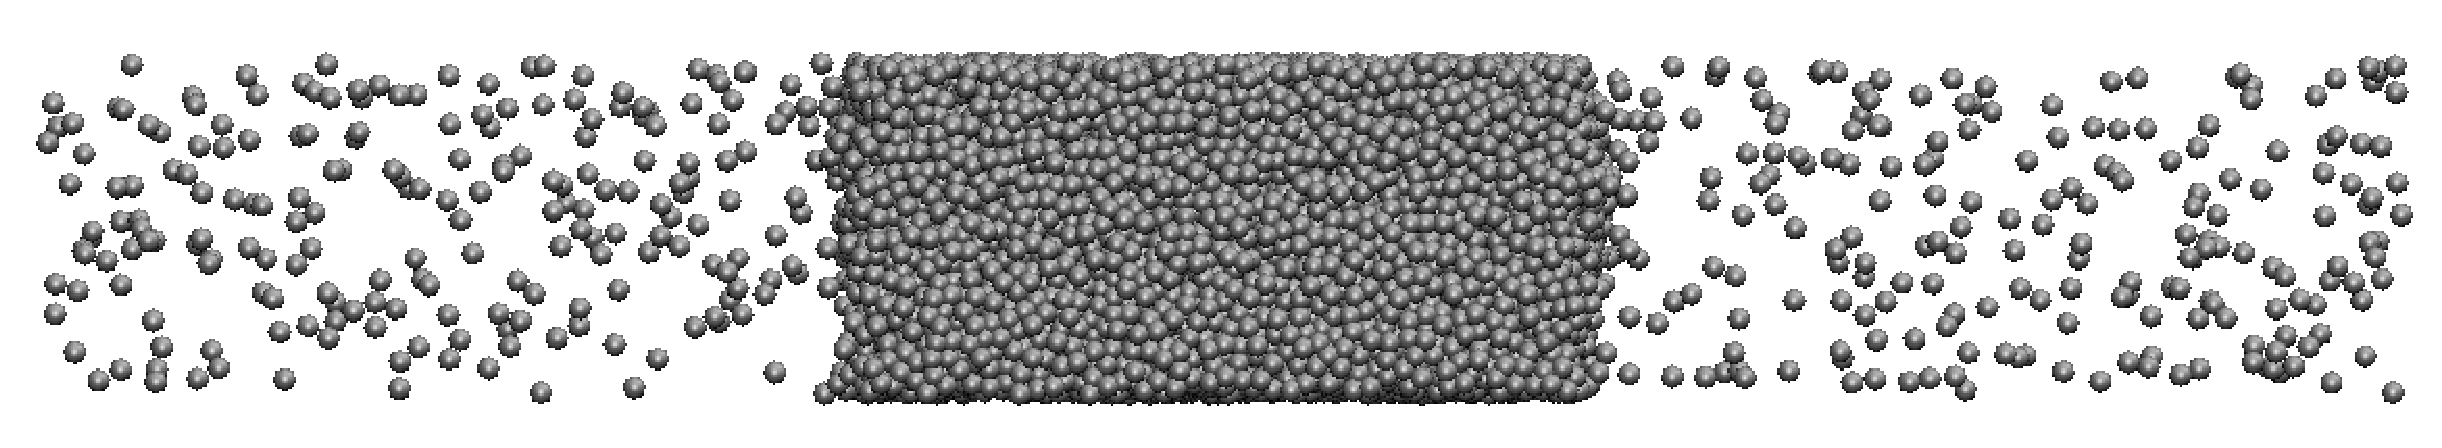
\includegraphics[width=0.9\textwidth]{fig/t0.85-n16000-rc07.5uni/confout.eps}
  \caption{The snapshot of the 16000 Lennard-Jones particle system at
    $T^\ast=0.85$ with a uniform cut-off radius of $r_c^\ast = 7.5$.}
  \label{fig:tmp1}
\end{figure}

\begin{figure}
  \centering
  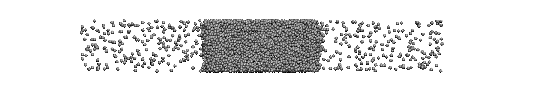
\includegraphics[]{fig/t0.85-n16000-rc07.5uni/confout-02.eps}
  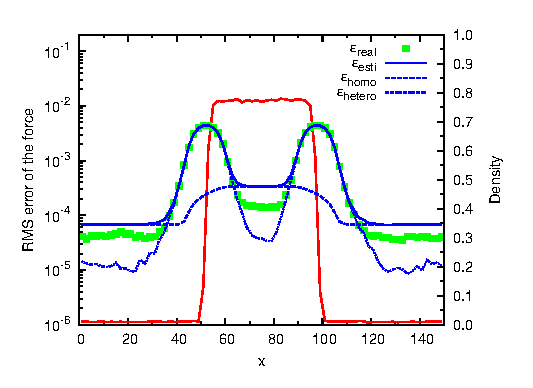
\includegraphics[]{fig/t0.85-n16000-rc07.5uni/error.uniform.eps}
  \caption{The error distribution of the 16000 Lennard-Jones particle
    system at $T^\ast=0.85$ with a uniform cut-off radius of $r_c^\ast
    = 7.5$.}
  \label{fig:tmp2}
\end{figure}

\begin{figure}
  \centering
  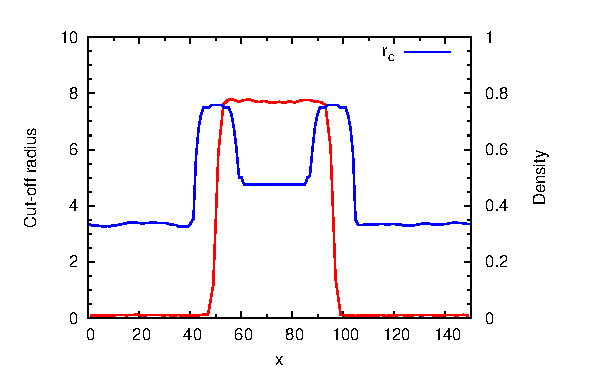
\includegraphics[]{fig/t0.85-n16000-adapt-e0.0045-extend/rcut.adapt.eps}
  \caption{The adapted cut-off radius of the 16000 Lennard-Jones
    particle system at $T^\ast=0.85$.}
  \label{fig:tmp2}
\end{figure}


\begin{figure}
  \centering
  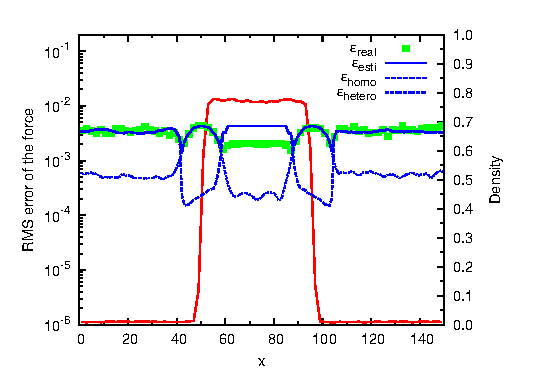
\includegraphics[]{fig/t0.85-n16000-adapt-e0.0045-extend/error.adapt.eps}
  \caption{The error distribution of the adaptive-cut-off 16000
    Lennard-Jones particle system at $T^\ast=0.85$.}
  \label{fig:tmp3}
\end{figure}


\begin{figure}
  \centering
  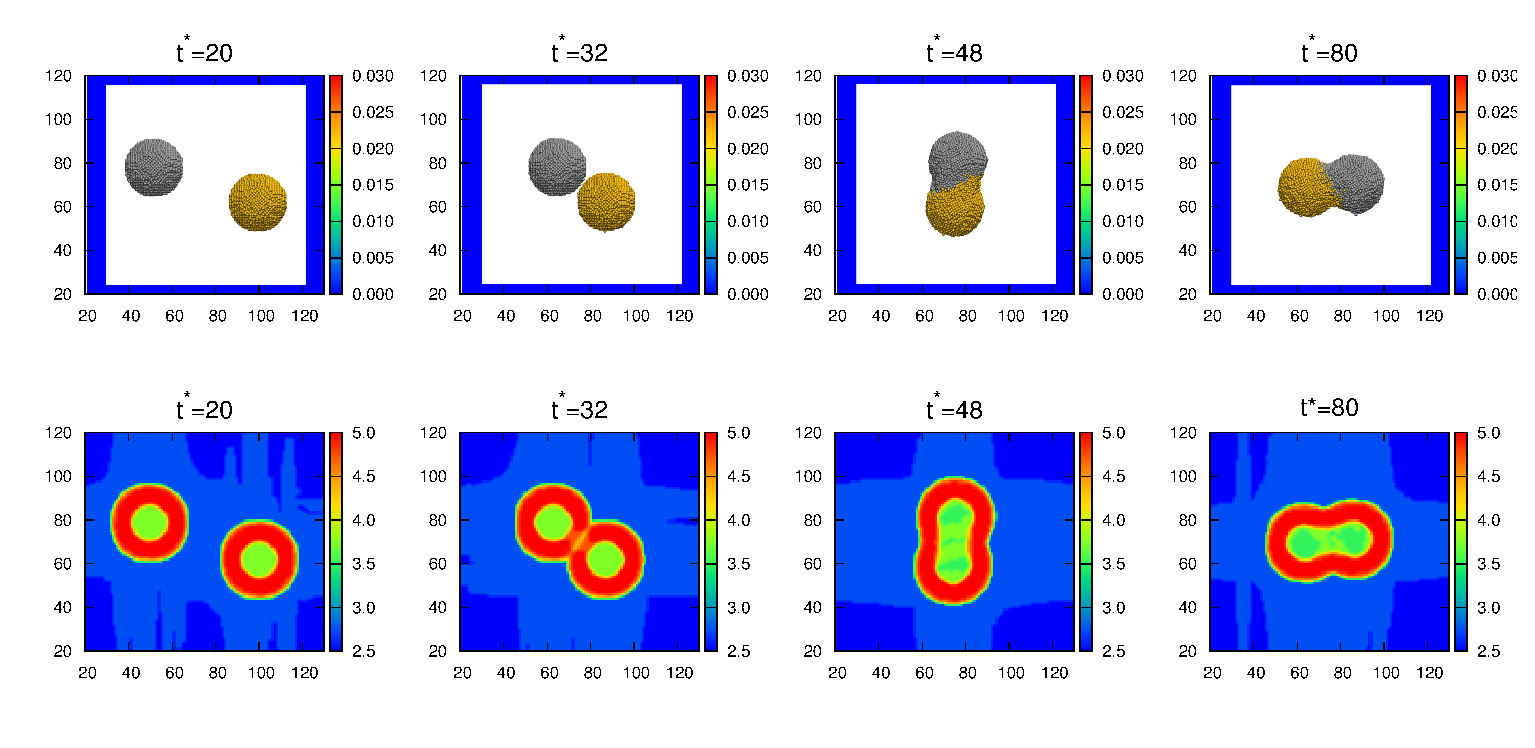
\includegraphics[width=0.90\textwidth]{fig/error-rcut-ball.eps} 
  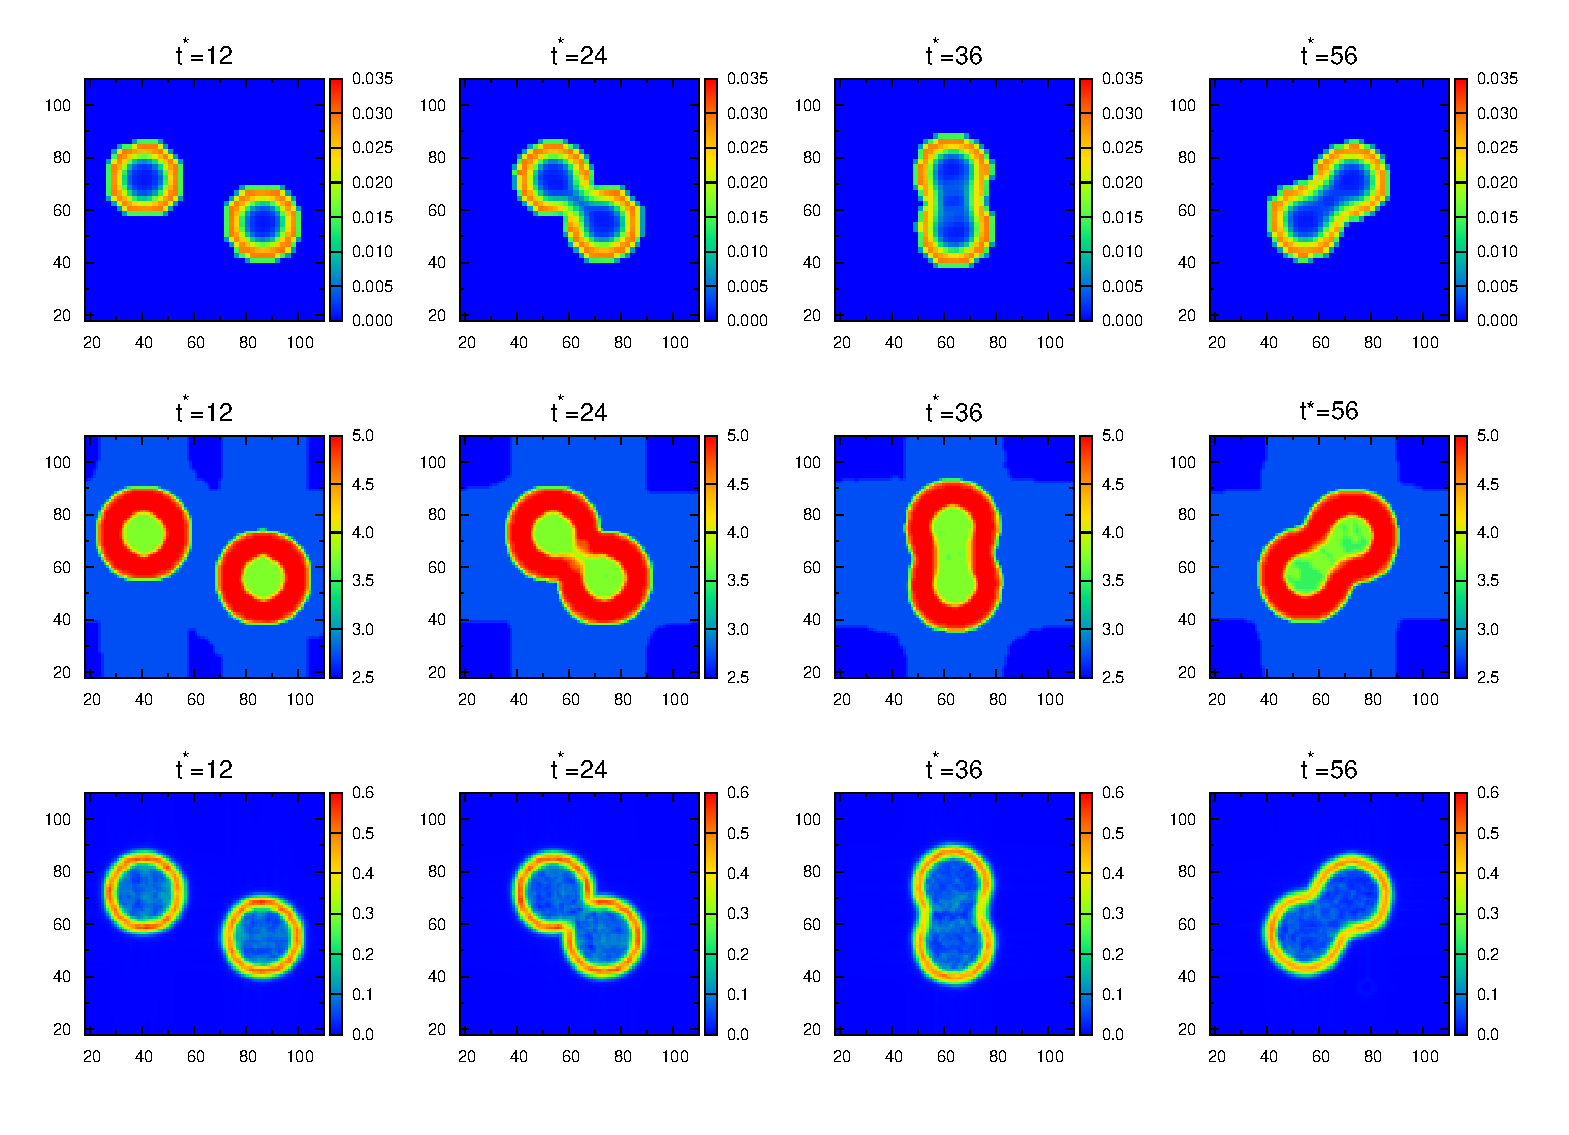
\includegraphics[width=0.90\textwidth]{fig/error-rcut.eps}
  \caption{normal words}
  \label{fig:tmp4}
\end{figure}

\begin{figure}
  \centering
  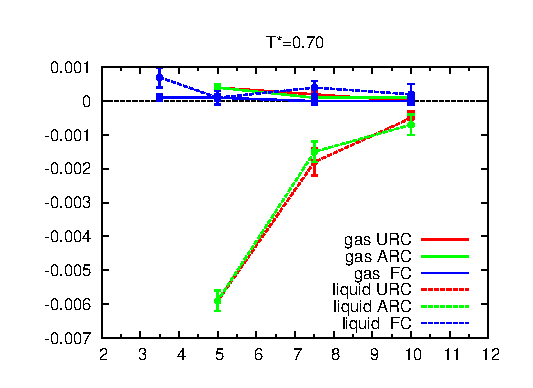
\includegraphics[width=0.49\textwidth]{fig/converge/t0.70.eps} 
  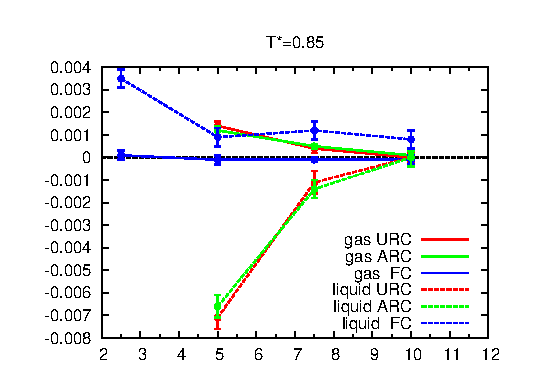
\includegraphics[width=0.49\textwidth]{fig/converge/t0.85.eps} 
  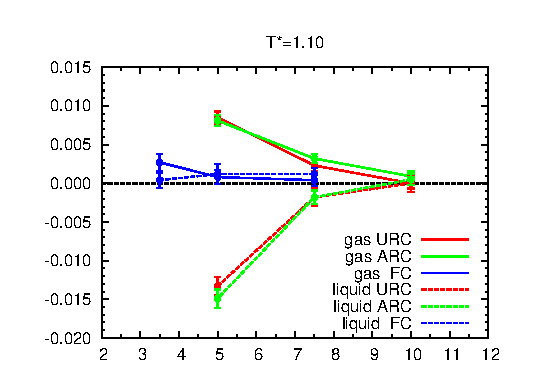
\includegraphics[width=0.49\textwidth]{fig/converge/t1.10.eps} 
  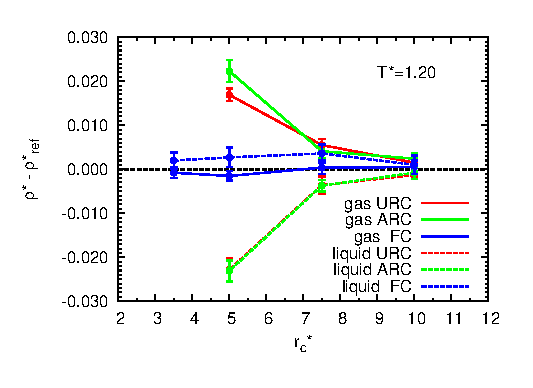
\includegraphics[width=0.49\textwidth]{fig/converge/t1.20.eps} 
  \caption{normal words}
  \label{fig:tmp4}
\end{figure}


\begin{figure}
  \centering
  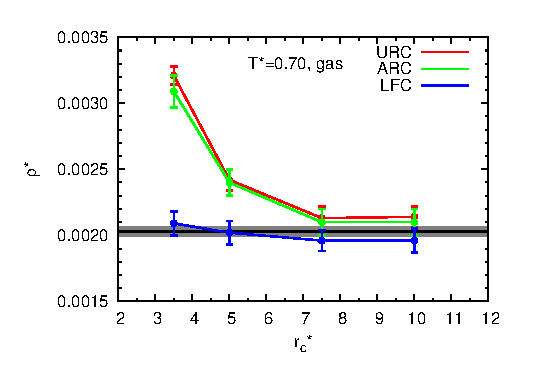
\includegraphics[width=0.46\textwidth]{fig/converge.new/t0.70.gas.eps} 
  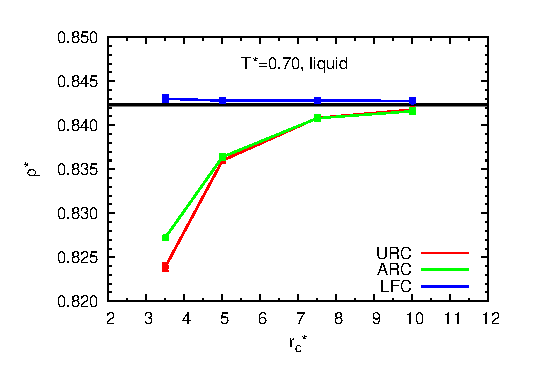
\includegraphics[width=0.46\textwidth]{fig/converge.new/t0.70.liquid.eps} 
  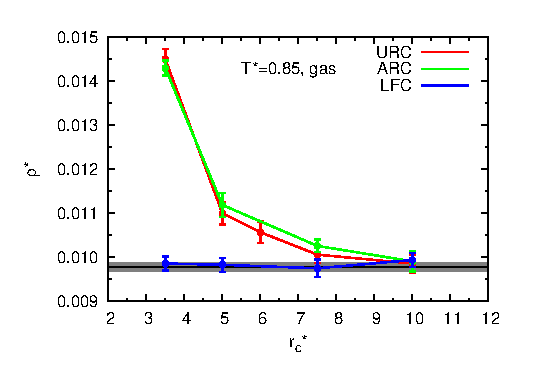
\includegraphics[width=0.46\textwidth]{fig/converge.new/t0.85.gas.eps} 
  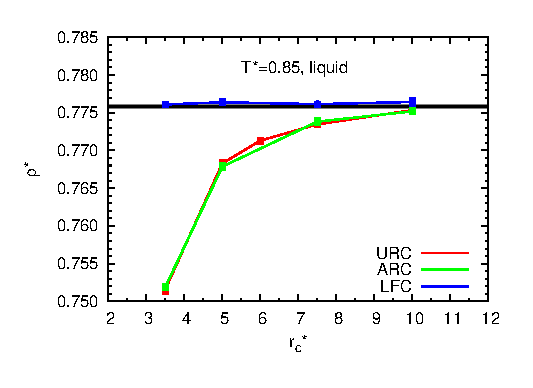
\includegraphics[width=0.46\textwidth]{fig/converge.new/t0.85.liquid.eps} 
  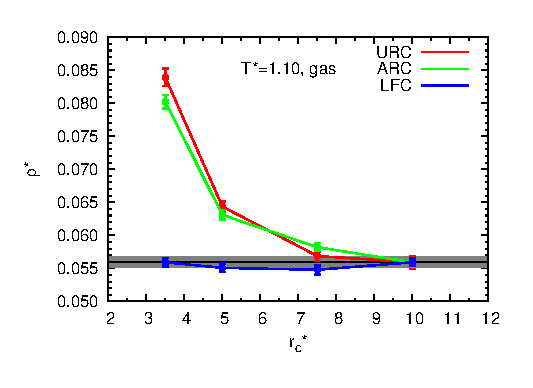
\includegraphics[width=0.46\textwidth]{fig/converge.new/t1.10.gas.eps} 
  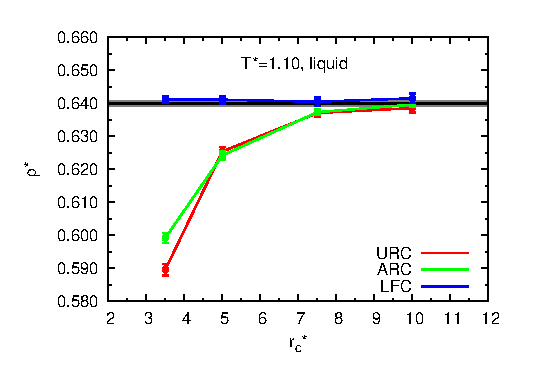
\includegraphics[width=0.46\textwidth]{fig/converge.new/t1.10.liquid.eps} 
  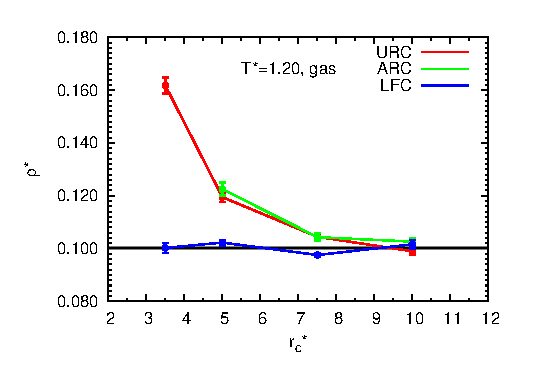
\includegraphics[width=0.46\textwidth]{fig/converge.new/t1.20.gas.eps} 
  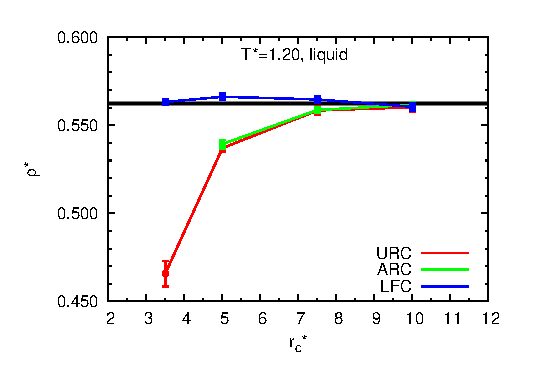
\includegraphics[width=0.46\textwidth]{fig/converge.new/t1.20.liquid.eps} 
  \caption{normal words}
  \label{fig:tmp4}
\end{figure}

\begin{figure}
  \centering
  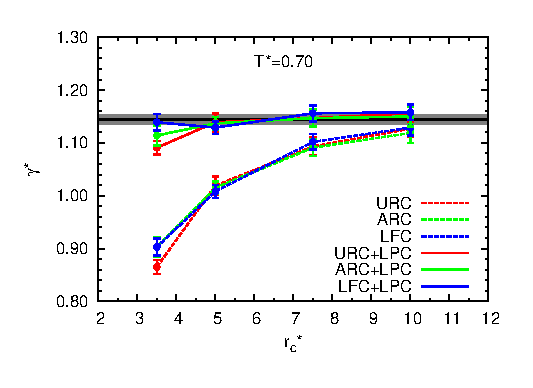
\includegraphics[width=0.49\textwidth]{fig/converge.new/tension.t0.70.eps} 
  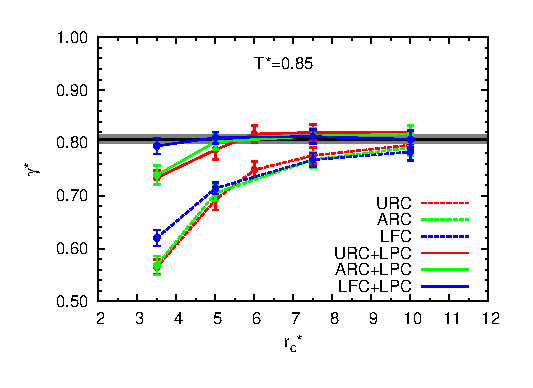
\includegraphics[width=0.49\textwidth]{fig/converge.new/tension.t0.85.eps} 
  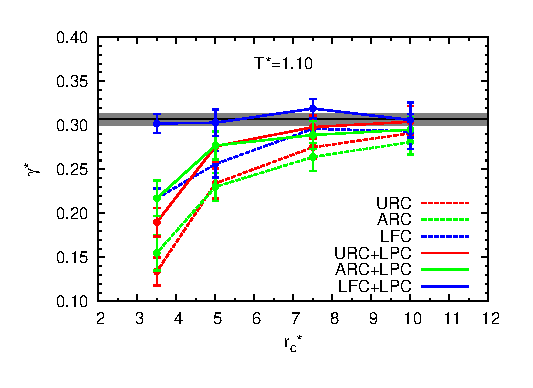
\includegraphics[width=0.49\textwidth]{fig/converge.new/tension.t1.10.eps} 
  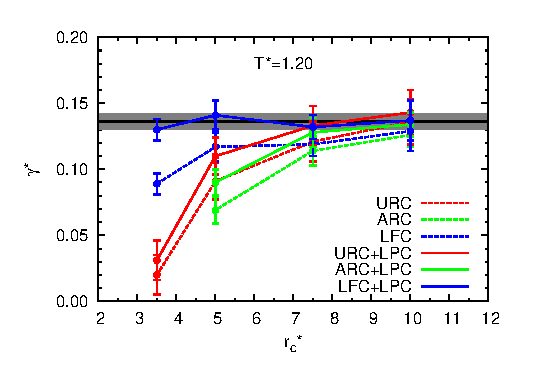
\includegraphics[width=0.49\textwidth]{fig/converge.new/tension.t1.20.eps} 
  \caption{The convergence of the surface tension with respect to the
    cut-off radius.  This figure presents the results of three
    methods, namely the uniform cut-off (URC), the adaptive cut-off
    (ARC) and the force correction (FC) method.  The results with and
    without heterogeneous pressure correction (HPC) are shown together
    for comparison. The reference surface tensions, shown by solid
    black lines, are measured by the uniform cut-off method with
    $r_c^\ast=13$ using HPC.}
\end{figure}




\begin{table}
  \centering
  \begin{tabular*}{0.99\textwidth}{c|c|@{\extracolsep{\fill}}clcccccc}\hline\hline
    $T^\ast$ & \textrm{method} &$r^\ast_{c}$ & $\mathcal E^\ast_{\textrm{target}}$  & $\rho^\ast_{\textrm{liq}}$ & $\rho^\ast_{\textrm{vap}}$ & $\gamma^\ast_{\textrm{sim}}$ & $\gamma^\ast_{\textrm{tail}}$ & $\gamma^\ast$ & cost\\\hline
    & \textrm{fcorr}  & 3.5     & -       & 0.0021 (1) & 0.8430 (3) & 0.898(18) & 0.238 & 1.135(18) & $3.4\times 10^6$\\\cline{2-10}
    & \textrm{unifom} & 5.0     & -       & 0.0024 (1) & 0.8364 (3) & 1.001(15) & 0.120 & 1.121(15) & $7.9\times 10^6$\\
    & \textrm{adapt}  & -       & 0.025   & 0.0024 (1) & 0.8364 (3) & 1.015(12) & 0.122 & 1.137(12) & $4.6\times 10^6$\\
    & \textrm{fcorr}  & 5.0     & -       & 0.0021 (1) & 0.8424 (2) & 1.024(11) & 0.121 & 1.145(11) & $8.8\times 10^6$\\\cline{2-10}
    & \textrm{unifom} & 7.5     & -       & 0.0022 (1) & 0.8405 (4) & 1.081(16) & 0.054 & 1.135(16) & $2.6\times 10^7$\\
0.70& \textrm{adapt}  & -       & 0.0050  & 0.0021 (1) & 0.8408 (3) & 1.091(16) & 0.056 & 1.147(16) & $1.3\times 10^7$\\
    & \textrm{fcorr}  & 7.5     & -       & 0.0020 (1) & 0.8427 (2) & 1.095(19) & 0.054 & 1.149(19) & $2.7\times 10^7$\\\cline{2-10}
    & \textrm{unifom} & 10.0    & -       & 0.0020 (1) & 0.8418 (2) & 1.125(12) & 0.029 & 1.154(12) & $5.9\times 10^7$\\
    & \textrm{adapt}  & -       & 0.0016  & 0.0021 (1) & 0.8416 (3) & 1.119(19) & 0.031 & 1.150(19) & $2.9\times 10^7$\\
    & \textrm{fcorr}  & 10.0    & -       & 0.0020 (1) & 0.8425 (3) & 1.121(16) & 0.029 & 1.149(16) & $5.9\times 10^7$\\\cline{2-10}
    & \textrm{unifom} & 11.5    & -       & 0.0020 (1) & 0.8422 (1) & 1.136(09) & 0.021 & 1.157(09) & $1.5\times 10^8$\\
    & \textrm{unifom} & 13.0    & -       & 0.0020 (0) & 0.8423 (2) & 1.128(10) & 0.016 & 1.144(10) & $2.1\times 10^8$\\\cline{2-10}
    & \textrm{ref}    & -       & -       & 0.0020 (0) & 0.8414 (1) & 1.081(11) & -     & 1.141(11) & - \\    \hline\hline
    & \textrm{fcorr}  & 3.5     & -       & 0.0097 (2) & 0.7765 (4) & 0.603(15) & 0.180 & 0.783(15) & $3.1\times 10^6$\\\cline{2-10}
    & \textrm{unifom} & 5.0     & -       & 0.0112 (2) & 0.7681 (5) & 0.707(14) & 0.094 & 0.801(14) & $7.1\times 10^6$\\
    & \textrm{adapt}  & -       & 0.022   & 0.0110 (2) & 0.7686 (5) & 0.697(16) & 0.094 & 0.791(16) & $4.6\times 10^6$\\
    & \textrm{fcorr}  & 5.0     & -       & 0.0098 (1) & 0.7760 (4) & 0.726(21) & 0.097 & 0.823(21) & $7.9\times 10^6$\\\cline{2-10}
    & \textrm{unifom} & 7.5     & -       & 0.0102 (2) & 0.7741 (5) & 0.776(15) & 0.044 & 0.819(15) & $2.4\times 10^7$\\
0.85& \textrm{adapt}  & -       & 0.0045  & 0.0103 (1) & 0.7738 (4) & 0.768(15) & 0.045 & 0.813(15) & $1.2\times 10^7$\\
    & \textrm{fcorr}  & 7.5     & -       & 0.0096 (2) & 0.7763 (5) & 0.763(13) & 0.044 & 0.807(13) & $2.4\times 10^7$\\\cline{2-10}
    & \textrm{unifom} & 10.0    & -       & 0.0098 (2) & 0.7752 (4) & 0.785(18) & 0.024 & 0.809(18) & $5.3\times 10^7$\\
    & \textrm{adapt}  & -       & 0.0015  & 0.0099 (2) & 0.7752 (4) & 0.791(16) & 0.026 & 0.817(16) & $2.6\times 10^7$\\
    & \textrm{fcorr}  & 10.0    & -       & 0.0097 (2) & 0.7762 (3) & 0.798(16) & 0.024 & 0.822(16) & $5.3\times 10^7$\\\cline{2-10}
    & \textrm{unifom} & 11.5    & -       & 0.0097 (1) & 0.7756 (2) & 0.800(06) & 0.017 & 0.818(06) & $1.3\times 10^8$\\
    & \textrm{unifom} & 13.0    & -       & 0.0098 (1) & 0.7758 (3) & 0.794(09) & 0.013 & 0.807(09) & $1.9\times 10^8$\\\cline{2-10}
    & \textrm{ref}    & -       & -       & 0.0098 (0) & 0.7750 (1) & 0.818(15) & -     & 0.818(15) & - \\    \hline\hline
  \end{tabular*}
\end{table}


\begin{table}
  \centering
  \begin{tabular*}{0.99\textwidth}{c|c|@{\extracolsep{\fill}}clcccccc}\hline\hline
    $T^\ast$ & \textrm{method} &$r^\ast_{c}$ & $\mathcal E^\ast_{\textrm{target}}$  & $\rho^\ast_{\textrm{liq}}$ & $\rho^\ast_{\textrm{vap}}$ & $\gamma^\ast_{\textrm{sim}}$ & $\gamma^\ast_{\textrm{tail}}$ & $\gamma^\ast$ & cost\\\hline
    & \textrm{fcorr}  & 3.5     & -       & 0.0535 (4) & 0.6422 (9) & 0.219(10) & 0.081 & 0.300(10) & $3.8\times 10^6$\\\cline{2-10}
    & \textrm{uniform}& 5.0     & -       & 0.0635 (8) & 0.6258(12) & 0.234(15) & 0.044 & 0.279(15) & $5.6\times 10^6$\\
    & \textrm{adapt}  & -       & 0.0160  & 0.0631 (7) & 0.6242(12) & 0.230(16) & 0.047 & 0.277(16) & $3.2\times 10^6$\\
    & \textrm{fcorr}  & 5.0     & -       & 0.0553 (6) & 0.6405 (9) & 0.247(09) & 0.046 & 0.293(09) & $9.9\times 10^6$\\\cline{2-10}
    & \textrm{uniform}& 7.5     & -       & 0.0573 (8) & 0.6373(11) & 0.281(12) & 0.023 & 0.303(12) & $1.7\times 10^7$\\
1.10& \textrm{adapt}  & -       & 0.0033  & 0.0582 (6) & 0.6373 (9) & 0.264(16) & 0.025 & 0.289(16) & $8.8\times 10^6$\\
    & \textrm{fcorr}  & 7.5     & -       & 0.0554 (8) & 0.6403 (8) & 0.294(17) & 0.022 & 0.317(17) & $1.8\times 10^7$\\\cline{2-10}
    & \textrm{uniform}& 10.0    & -       & 0.0550 (7) & 0.6391(11) & 0.300(16) & 0.013 & 0.313(16) & $3.9\times 10^7$\\
    & \textrm{adapt}  & -       & 0.0011  & 0.0559 (6) & 0.6396 (7) & 0.280(14) & 0.014 & 0.295(14) & $1.9\times 10^7$\\
    & \textrm{fcorr}  & 10.0    & -       & 0.0549 (8) & 0.6401 (8) & 0.295(19) & 0.013 & 0.308(19) & $3.9\times 10^7$\\\cline{2-10}
    & \textrm{uniform}& 11.5    & -       & 0.0558 (6) & 0.6395 (4) & 0.297(06) & 0.009 & 0.307(06) & $9.9\times 10^7$\\
    & \textrm{uniform}& 13.0    & -       & 0.0560 (8) & 0.6399 (9) & 0.300(07) & 0.007 & 0.307(07) & $1.4\times 10^8$\\\cline{2-10}
    & \textrm{ref}    & -       & -       & 0.0553 (0) & 0.6383 (1) & 0.302(11) & -     & 0.302(11) & - \\    \hline\hline
    & \textrm{fcorr}  & 3.5     & -       & 0.0994(12) & 0.5644(18) & 0.096(13) & 0.042 & 0.137(13) & $1.8\times 10^6$\\\cline{2-10}
    & \textrm{uniform}& 5.0     & -       & 0.1171(14) & 0.5396(26) & 0.074(17) & 0.019 & 0.093(17) & $4.2\times 10^6$\\
    & \textrm{adapt}  & -       & 0.0098  & 0.1218(19) & 0.5415(23) & 0.085(12) & 0.021 & 0.106(12) & $2.9\times 10^6$\\
    & \textrm{fcorr}  & 5.0     & -       & 0.0987(11) & 0.5651(22) & 0.110(17) & 0.026 & 0.136(17) & $4.6\times 10^6$\\\cline{2-10}
    & \textrm{uniform}& 7.5     & -       & 0.1057(14) & 0.5588(20) & 0.120(16) & 0.012 & 0.132(16) & $1.4\times 10^7$\\
1.20& \textrm{adapt}  & -       & 0.0024  & 0.1043(15) & 0.5587(13) & 0.114(11) & 0.014 & 0.128(11) & $7.7\times 10^6$\\
    & \textrm{fcorr}  & 7.5     & -       & 0.1006(16) & 0.5660(21) & 0.127(10) & 0.013 & 0.140(10) & $1.4\times 10^7$\\\cline{2-10}
    & \textrm{uniform}& 10.0    & -       & 0.1014 (6) & 0.5614(12) & 0.127(08) & 0.007 & 0.135(08) & $3.0\times 10^7$\\
    & \textrm{adapt}  & -       & 0.00082 & 0.1026(12) & 0.5616(14) & 0.125(09) & 0.008 & 0.134(09) & $1.7\times 10^7$\\
    & \textrm{fcorr}  & 10.0    & -       & 0.1007(15) & 0.5634(21) & 0.118(12) & 0.008 & 0.125(12) & $3.1\times 10^7$\\\cline{2-10}
    & \textrm{uniform}& 11.5    & -       & 0.1013 (8) & 0.5612 (8) & 0.128(06) & 0.006 & 0.133(06) & $7.9\times 10^7$\\
    & \textrm{uniform}& 13.0    & -       & 0.1002 (5) & 0.5624(11) & 0.131(06) & 0.004 & 0.136(06) & $1.1\times 10^8$\\\cline{2-10}
    & \textrm{ref}    & -       & -       & 0.0942 (0) & 0.5627 (2) & 0.156(14) & -     & 0.156(14) & - \\    \hline    \hline    
  \end{tabular*}
\end{table}


 \newpage

% \bibliography{ref}{}
% \bibliographystyle{unsrt}

\begin{table}
  \centering
  \begin{tabular*}{0.99\textwidth}{@{\extracolsep{\fill}}cclllllc}\hline\hline
  % \begin{tabular}{cccc|cccc}\hline\hline
    $T^\ast$ & Method & Model & $r_c^\ast$ & $\rho^\ast_{\textrm{liq}}$ & $\rho^\ast_{\textrm{vap}}$ & $\gamma^\ast$ & Source \\\hline
    0.70 & MC & ST & 2.5 & 0.807 & 0.004  & 1.28  & \cite{chapela1977computer}\\
    0.70 & MC & ST & 2.5 & 0.812 & 0.0029 & 0.640 & \cite{trokhymchuk1999computer} \\
    0.70 & MD & STS& 2.5 & 0.788 & 0.010  & 1.12  & \cite{chapela1977computer}\\
    0.70 & MD & STS& 2.5 & 0.7852 & 0.0067 & 0.610 & \cite{trokhymchuk1999computer}\\
    0.70 & MD & HLRC & 5.0 & 0.8375 & 0.00201 & 1.1394(193) & \cite{mecke1997molecular}\\
    0.70 & MC & HLRC & 2.5 & 0.842(1) & 0.0021(2) & 1.21(2) & \cite{janecek2006long}\\
    0.70 & MD & Npt+test particle & 5.0 & 0.84266(18) & 0.00193(10) & & \cite{lotfi1992vapour}\\
    0.70 & MC & GC-TMMC & 1/2 box & 0.8424(13) & 0.001992(2) & 1.182(10) & \cite{errington2003evaluating}\\
    0.70 & MD & Ewald & 5.0(real) & 0.8414(1) & 0.0020(0) & 1.141(11) & \cite{ismail2007application}\\
    0.70 & MD & HLRC & 5.0 & 0.8424(2) & 0.0021(1) & 1.145(11) & this work\\\hline
    0.85 & MD & HLRC & 5.0 & 0.7698 & 0.00977 & 0.7927(172) & \cite{mecke1997molecular}\\
    0.85 & MD & Npt+test particle & 5.0 & 0.77623(25) & 0.00970(22) & & \cite{lotfi1992vapour}\\
    0.85 & MC & GC-TMMC & 1/2 box & 0.7760(10) & 0.009611(9) & 0.837(2) & \cite{errington2003evaluating}\\
    0.85 & MD & Ewald & 5.0(real) & 0.7750(1) & 0.0098(0) & 0.818(15) & \cite{ismail2007application}\\
    0.85 & MD & HLRC & 5.0 & 0.7760(4) & 0.0098(1) & 0.823(21) & this work\\\hline
    1.10 & MD & HLRC & 5.0 & 0.6236 & 0.05937 & 0.3193(139) & \cite{mecke1997molecular}\\
    1.10 & MC & HLRC & 2.5 & 0.642(1) & 0.054(1) & 0.33(2) & \cite{janecek2006long}\\
    1.10 & MC & GC-TMMC & 1/2 box & 0.6410(7) & 0.05485(5) & 0.343(2) & \cite{errington2003evaluating}\\
    1.10 & MD & Npt+test particle & 5.0 & 0.6401(12) & 0.0533(14) && \cite{lotfi1992vapour}\\
    1.10 & MD & Ewald & 3.5(real) & 0.6370 & 0.0541 & 0.31(2) & \cite{lopez2002thermodynamic}\\
    1.10 & MD & Ewald & 5.0(real) & 0.6383(1) & 0.0553(0) & 0.302(11) & \cite{ismail2007application}\\
    1.10 & MD & HLRC & 5.0 & 0.6405(9) & 0.0553(6) & 0.293(9) & this work\\
    \hline\hline
  % \end{tabular}
  \end{tabular*}
  \caption{Comparision of previous results}
  \label{tab:tmp5}
\end{table}


\begin{table}
  \centering
  \caption{Equilibrium densities and surface tension comparision 
    with various literature results: Monte Carlo with long-range
    energy correction (MC/LEC)~\cite{janecek2006long}, Npt+test
    particle molecular dynamics (MD/Npt+test particle)~\cite{lotfi1992vapour},
    grand-canonical transition-matrix Monte Carlo (MC/GC-TMMC)~\cite{errington2003evaluating},
    molecular dynamics with dispersion term calculated by the Ewald
    summation (MD/Ewald)~\cite{ismail2007application}
    and uniform cut-off (URC) and long-range force correction (LFC) molecular dynamics
    proposed by this work. The surface tensions of this work are
    corrected by the long-range pressure correction.
    The cut-off radius of the Ewald summation is for the real space.
  }
  \label{tab:comparison}
  \begin{tabular*}{0.99\textwidth}{@{\extracolsep{\fill}}clllllc}\hline\hline
  % \begin{tabular}{cccc|cccc}\hline\hline
    $T^\ast$ & Method & $r_c^\ast$ & $\rho^\ast_{\textrm{liq}}$ & $\rho^\ast_{\textrm{vap}}$ & $\gamma^\ast$ & Source \\\hline
    0.70 & MC/LEC               & 2.5      & 0.842(1)    & 0.0021(2)   & 1.21(2)   & \cite{janecek2006long}\\
    0.70 & MD/Npt+test particle & 5.0      & 0.84266(18) & 0.00193(10) & -         & \cite{lotfi1992vapour}\\
    0.70 & MC/GC-TMMC           & 1/2 box  & 0.8424(13)  & 0.001992(2) & 1.182(10) & \cite{errington2003evaluating}\\
    % 0.70 & MD/Ewald             & 5.0(real)& 0.8414(1)   & 0.0020(0)   & 1.141(11) & \cite{ismail2007application}\\
    0.70 & MD/URC               & 13.0     & 0.8423(2)   & 0.0020(0)   & 1.128(10) & this work \\
    % 0.70 & MD/LFC               & 5.0      & 0.8424(2)   & 0.0021(1)   & 1.145(11) & this work \\\hline
    0.70 & MD/LFC               & 3.5      & 0.8430(4)   & 0.00209(9)  & 1.139(16) & this work \\\hline
    0.85 & MD/Npt+test particle & 5.0      & 0.77623(25) & 0.00970(22) & -         & \cite{lotfi1992vapour}\\
    0.85 & MC/GC-TMMC           & 1/2 box  & 0.7760(10)  & 0.009611(9) & 0.837(2)  & \cite{errington2003evaluating}\\
    % 0.85 & MD/Ewald             & 5.0(real)& 0.7750(1)   & 0.0098(0)   & 0.818(15) & \cite{ismail2007application}\\
    0.85 & MD/URC               & 13.0     & 0.7758(3)   & 0.0098(1)   & 0.794(09) & this work \\
    % 0.85 & MD/LFC               & 5.0      & 0.7760(4)   & 0.0098(1)   & 0.823(21) & this work\\\hline
    0.85 & MD/LFC               & 3.5      & 0.7761(3)   & 0.00986(16) & 0.794(15) & this work\\\hline
    1.10 & MC/LEC               & 2.5      & 0.642(1)    & 0.054(1)    & 0.33(2)   & \cite{janecek2006long}\\
    1.10 & MD/Npt+test particle & 5.0      & 0.6401(12)  & 0.0533(14)  & -         & \cite{lotfi1992vapour}\\
    1.10 & MC/GC-TMMC           & 1/2 box  & 0.6410(7)   & 0.05485(5)  & 0.343(2)  & \cite{errington2003evaluating}\\
    % 1.10 & MD/Ewald             & 5.0(real)& 0.6383(1)   & 0.0553(0)   & 0.302(11) & \cite{ismail2007application}\\
    1.10 & MD/URC               & 13.0     & 0.6399(9)   & 0.0560(8)   & 0.300(07) & this work\\
    % 1.10 & MD/LFC               & 5.0      & 0.6405(9)   & 0.0553(6)   & 0.293(9)  & this work\\ \hline
    1.10 & MD/LFC               & 3.5      & 0.6411(10)   & 0.0559(6)   & 0.302(11)  & this work\\ \hline
    1.20 & MC/LEC               & 2.5      & 0.566(1)    & 0.109(2)    & 0.16(2)   & \cite{janecek2006long}\\
    1.20 & MD/Npt+test particle & 5.0      & 0.5661(22)  & 0.0987(16)  & -         & \cite{lotfi1992vapour}\\
    % 1.20 & MD/Ewald             & 5.0(real)& 0.5627(2)   & 0.0942(0)   & 0.156(14) & \cite{ismail2007application}\\
    1.20 & MD/URC               & 13.0     & 0.5624(11)  & 0.1002(5)   & 0.131(6) & this work\\
    % 1.20 & MD/LFC               & 5.0      & 0.5651(22)  & 0.0987(11)  & 0.136(17) & this work\\
    1.20 & MD/LFC               & 3.5      & 0.5632(14)  & 0.1002(19)  & 0.130(8) & this work\\
    \hline\hline
  % \end{tabular}
  \end{tabular*}
\end{table}


\bibliography{ref}{}
\bibliographystyle{unsrt}



\end{document}
